\subsection*{Log ind}
Log ind-funktionen inddeles i en klasse af typen boundary samt en tilhørende controller. Disse fremgår af \autoref{fig:Designlogind}. 

\begin{figure} [H]
\centering
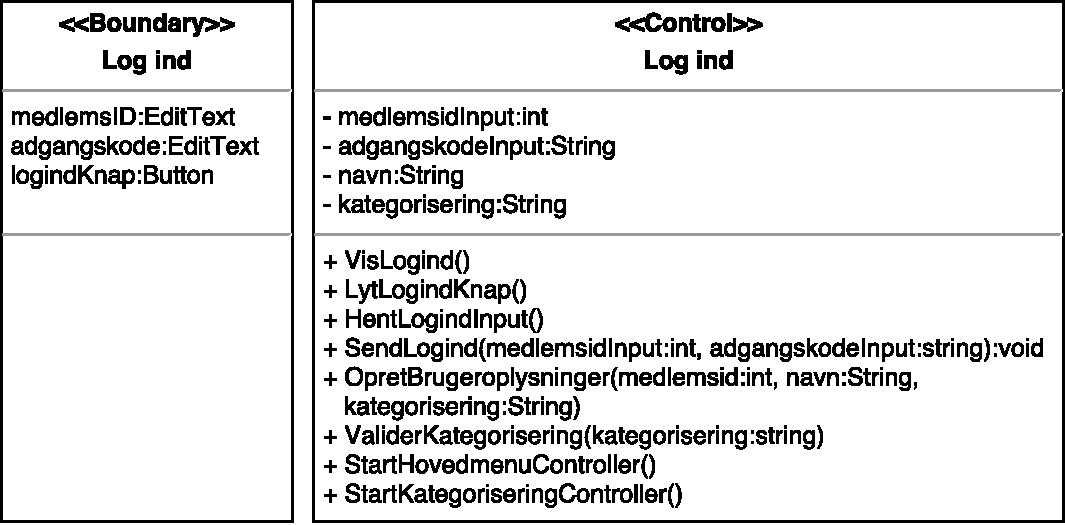
\includegraphics[width=0.9\textwidth]{figures/MVC/MVCLogInd}
\caption{Designklasser for log ind. Til venstre ses grænsefladen og til højre den tilhørende controller.}
\label{fig:Designlogind}
\end{figure}

\noindent
I grænsefladen for \textit{Logind} opstilles tekstfelter af typen EditText, hvor brugeren kan angive medlemsID samt adgangskode. Dertil opsættes en LogindKnap, af typen Button, der ved tryk indikerer, at brugerens informationer er angivet og klar til at logge ind. 

Til denne grænseflade er der opstillet en \textit{Logind} controller. Denne controller har metoderne Vis, Lyt, Hent, Valider, Opret og Start. Controlleren validerer log ind og opretter tre entitys, hvori oplysninger senere kan lagres. Disse entitys beskrives af \autoref{sec:entity}. Ligeledes håndterer controlleren, hvilken grænseflade systemet efterfølgende skal henvises til. Der er i sammenspil med disse designklasser udarbejdet et sekvensdiagram, der fremgår af \autoref{fig:SEKlogind}.

\begin{figure} [H]
\centering
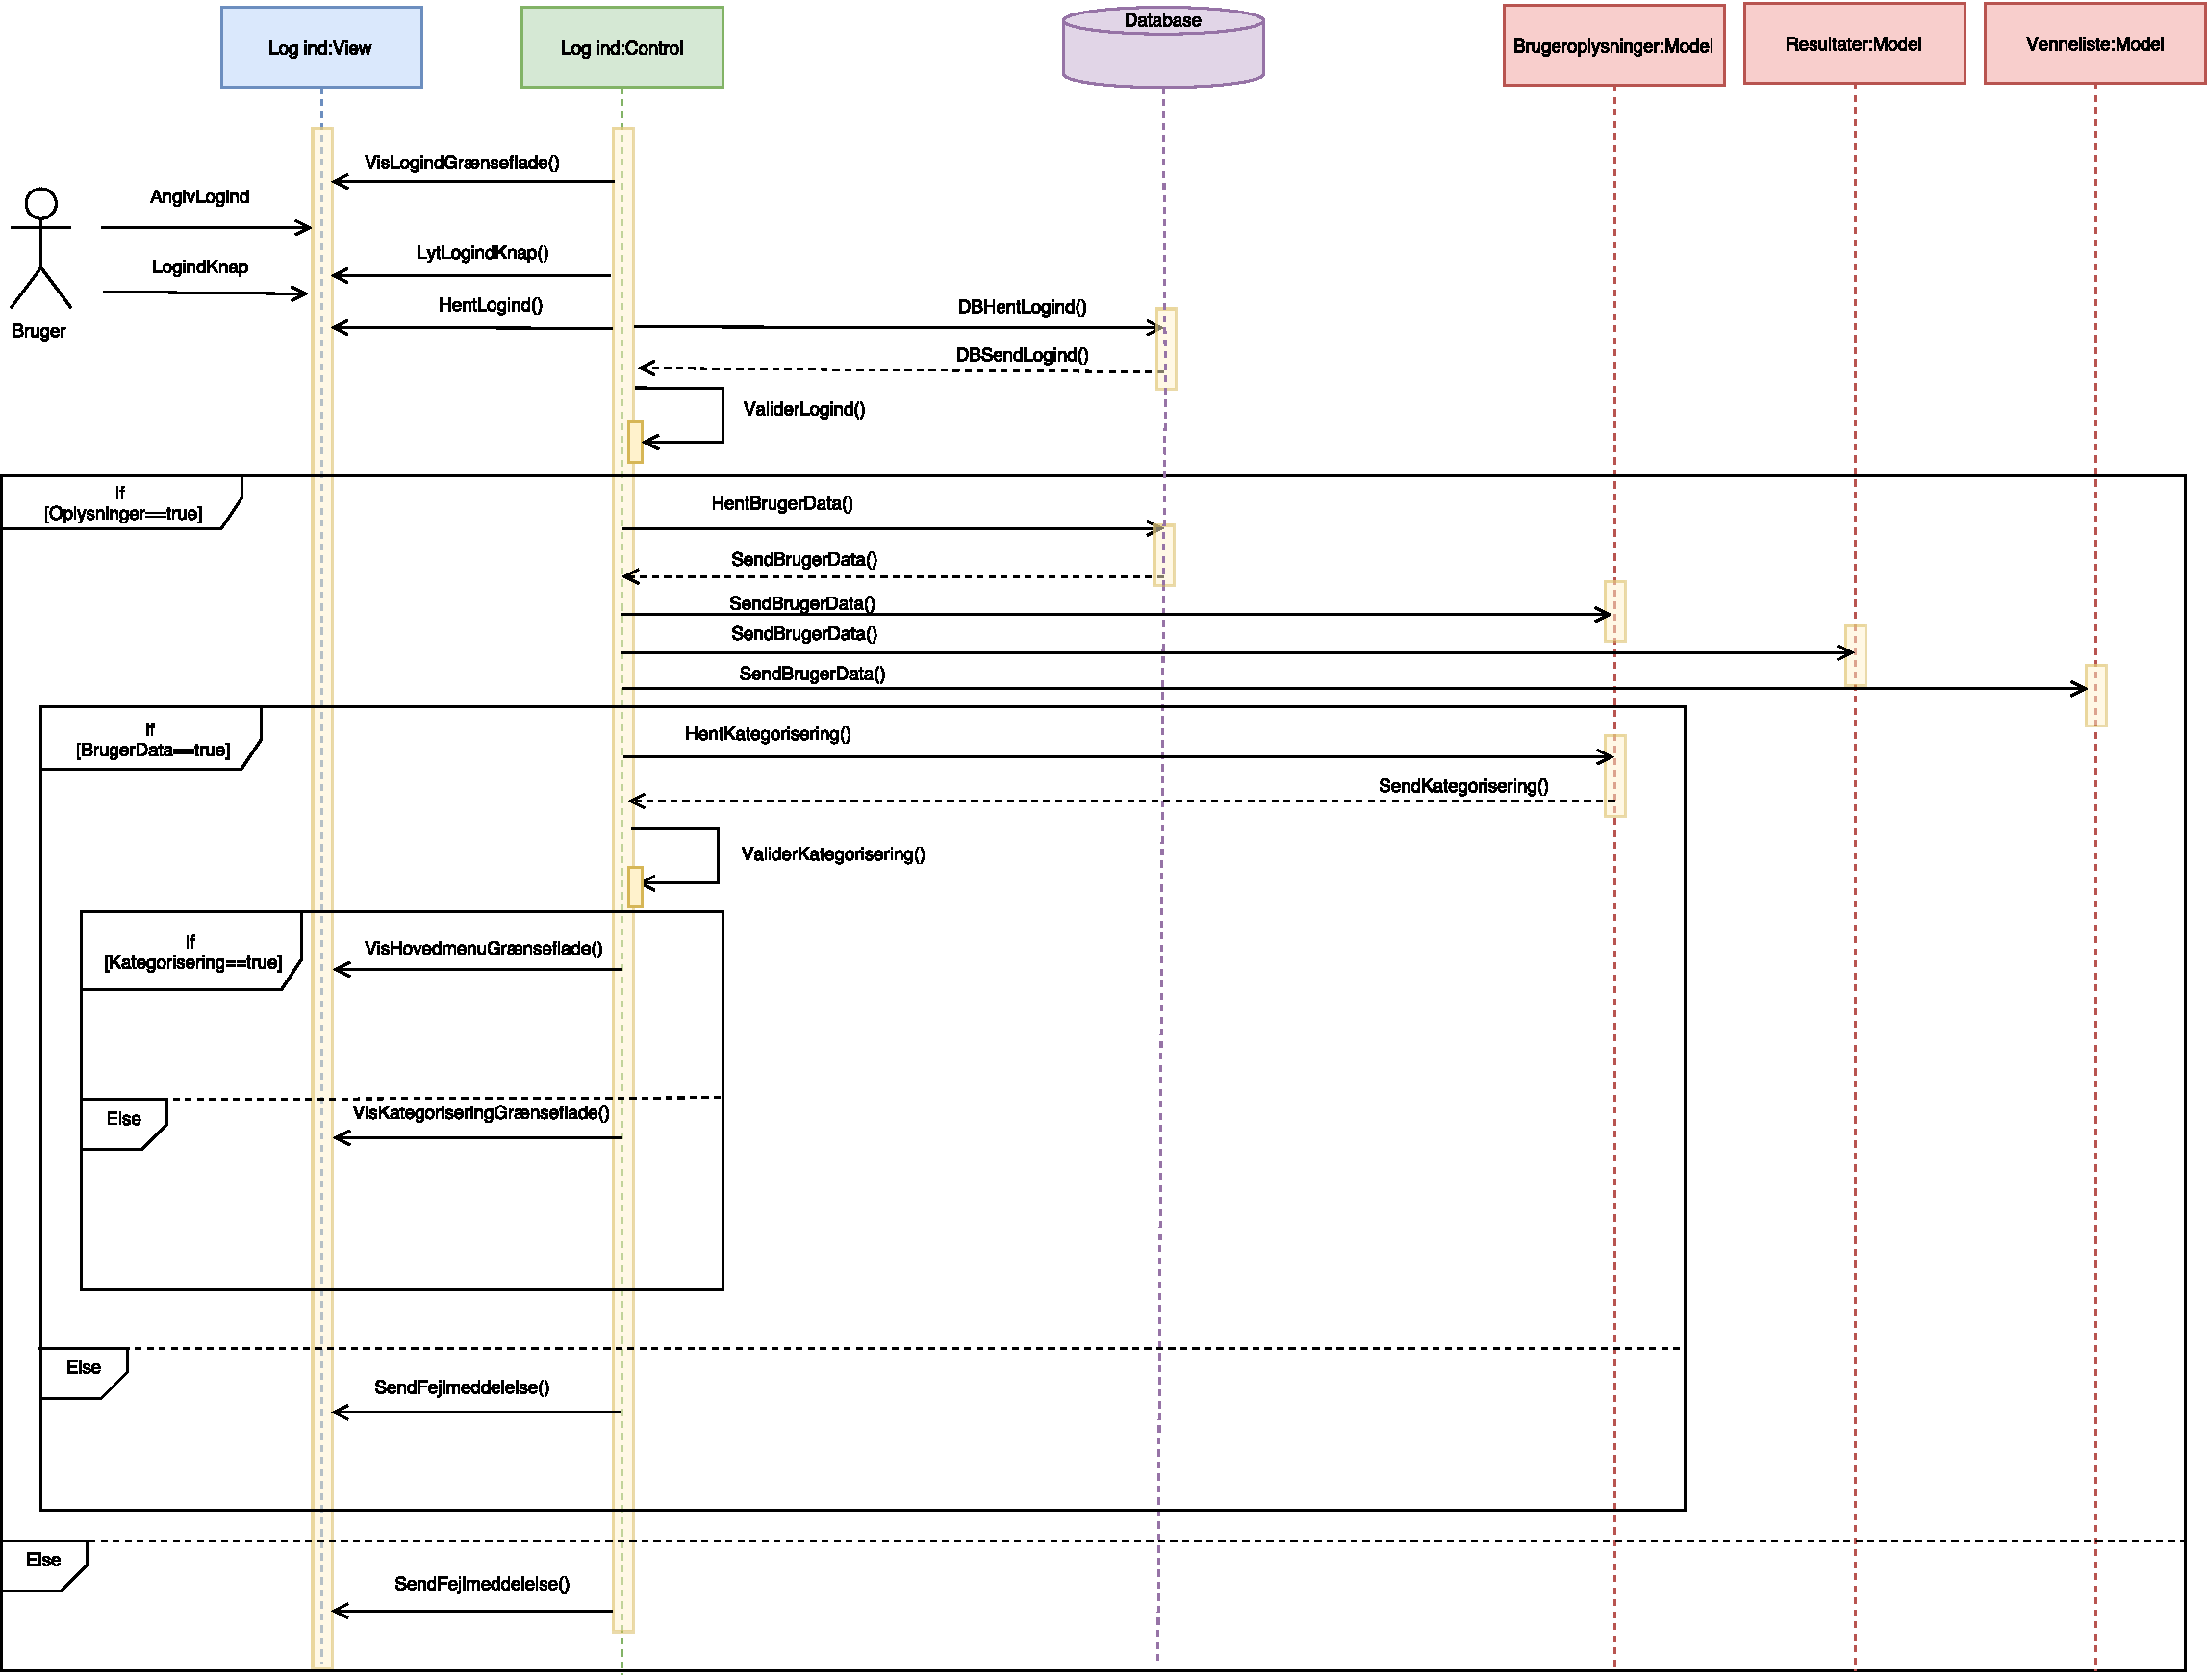
\includegraphics[width=1.55\textwidth, angle=90]{figures/Sek/SEKLogInd}
\caption{Sekvensdiagram for log ind.}
\label{fig:SEKlogind}
\end{figure}

\noindent
Det fremgår af sekvensdiagrammet, at controlleren for \textit{Log ind} starter med at vise grænsefladen for \textit{Log ind}. Dertil lytter controlleren på LogindKnap, der ved tryk henter brugerens angivne log ind-informationer. Contolleren henter ligeledes log ind-informationer passende til det indtastede medlemsID i databasen, hvorefter log ind valideres. Bekræftes log ind oprettes en entity af \textit{Brugeroplysninger}, der henter og lagrer brugeroplysninger fra databasen. Forefindes en kategorisering i disse oplysninger, oprettes to yderligere entitys, der omfatter \textit{KonditionResultater} og \textit{Venneliste}. \fxnote{Måske et dårligt designvalg, der vil stadig skulle hentes meget information} Disse entitys henter og lagrer ligeledes deres respektive data fra databasen. Systemet henvises hertil til hovedmenu, der fremgår af \autoref{fig:SEKHovedmenu}.
Forekommer ingen kategorisering i \textit{Brugeroplysninger}, oprettes de to entitys, \textit{KonditionResultater} og \textit{Venneliste}, dog uden at hente og lagre data fra databasen. Systemet henvises herefter til kategoriseringen, hvilket er illustreret af \autoref{fig:SEKKate}.
Mislykkes log ind, vises en fejlmeddelelse til \textit{Log ind} grænsefladen, hvorved brugeren igen kan indtaste sit log ind.
